\documentclass[notes,11pt, aspectratio=169]{beamer}

\usepackage{pgfpages}
% These slides also contain speaker notes. You can print just the slides,
% just the notes, or both, depending on the setting below. Comment out the want
% you want.
\setbeameroption{hide notes} % Only slide
%\setbeameroption{show only notes} % Only notes
%\setbeameroption{show notes on second screen=right} % Both

%\usepackage[scaled=1.0]{helvet}
\usepackage{array}


\usepackage{tikz}
\usetikzlibrary{calc}
\usetikzlibrary{matrix}
\usetikzlibrary{positioning}

\newcommand{\payoff}[4][below]{\node[#1]at(#2){$(#3,#4)$};}
\usepackage{verbatim}
\setbeamertemplate{note page}{\pagecolor{gray!5}\insertnote}
\usetikzlibrary{positioning}
\usetikzlibrary{snakes}
\usetikzlibrary{calc}
\usetikzlibrary{arrows}
\usetikzlibrary{decorations.markings}
\usetikzlibrary{shapes.misc}
\usetikzlibrary{matrix,shapes,arrows,fit,tikzmark}
\usepackage{amsmath}
\usepackage{mathpazo}
\usepackage{hyperref}
\usepackage{lipsum}
\usepackage{multimedia}
\usepackage{graphicx}
\usepackage{multirow}
\usepackage{graphicx}
\usepackage{dcolumn}
\usepackage{bbm}
\newcolumntype{d}[0]{D{.}{.}{5}}

\usepackage{changepage}
\usepackage{appendixnumberbeamer}
\newcommand{\beginbackup}{
   \newcounter{framenumbervorappendix}
   \setcounter{framenumbervorappendix}{\value{framenumber}}
   \setbeamertemplate{footline}
   {
     \leavevmode%
     \hline
     box{%
       \begin{beamercolorbox}[wd=\paperwidth,ht=2.25ex,dp=1ex,right]{footlinecolor}%
%         \insertframenumber  \hspace*{2ex} 
       \end{beamercolorbox}}%
     \vskip0pt%
   }
 }
\newcommand{\backupend}{
   \addtocounter{framenumbervorappendix}{-\value{framenumber}}
   \addtocounter{framenumber}{\value{framenumbervorappendix}} 
}


\usepackage{graphicx}
\usepackage[space]{grffile}
\usepackage{booktabs}

% These are my colors -- there are many like them, but these ones are mine.
\definecolor{blue}{RGB}{0,114,178}
\definecolor{red}{RGB}{213,94,0}
\definecolor{yellow}{RGB}{240,228,66}
\definecolor{green}{RGB}{0,158,115}

\hypersetup{
  colorlinks=false,
  linkbordercolor = {white},
  linkcolor = {blue}
}

\usepackage{graphicx,stackengine,xcolor}
\newcommand\Circle[1]{%
	\def\useanchorwidth{T}%
	\def\stacktype{L}%
	\stackon[0pt]{#1}{\scalebox{2.0}[1.15]{\textcolor{red}{$\bigcirc$}}}%
}

%% I use a beige off white for my background
\definecolor{MyBackground}{RGB}{255,253,218}

%% Uncomment this if you want to change the background color to something else
%\setbeamercolor{background canvas}{bg=MyBackground}

%% Change the bg color to adjust your transition slide background color!
\newenvironment{transitionframe}{
  \setbeamercolor{background canvas}{bg=white}
  \begin{frame}}{
    \end{frame}
}

\setbeamercolor{frametitle}{fg=blue}
\setbeamercolor{title}{fg=black}
\setbeamertemplate{footline}[frame number]
\setbeamertemplate{navigation symbols}{} 
\setbeamertemplate{itemize items}{-}
\setbeamercolor{itemize item}{fg=blue}
\setbeamercolor{itemize subitem}{fg=blue}
\setbeamercolor{enumerate item}{fg=blue}
\setbeamercolor{enumerate subitem}{fg=blue}
\setbeamercolor{button}{bg=MyBackground,fg=blue,}

%%% TIKZ STUFF
\tikzset{   
	every picture/.style={remember picture,baseline},
	every node/.style={anchor=base,align=center,outer sep=1.5pt},
	every path/.style={thick},
}
\newcommand\marktopleft[1]{%
	\tikz[overlay,remember picture] 
	\node (marker-#1-a) at (-.3em,.3em) {};%
}
\newcommand\markbottomright[2]{%
	\tikz[overlay,remember picture] 
	\node (marker-#1-b) at (0em,0em) {};%
}
\tikzstyle{every picture}+=[remember picture] 
\tikzstyle{mybox} =[draw=black, very thick, rectangle, inner sep=10pt, inner ysep=20pt]
\tikzstyle{fancytitle} =[draw=black,fill=red, text=white]
%%%% END TIKZ STUFF


% If you like road maps, rather than having clutter at the top, have a roadmap show up at the end of each section 
% (and after your introduction)
% Uncomment this is if you want the roadmap!
% \AtBeginSection[]
% {
%    \begin{frame}
%        \frametitle{Roadmap of Talk}
%        \tableofcontents[currentsection]
%    \end{frame}
% }
\setbeamercolor{section in toc}{fg=blue}
\setbeamercolor{subsection in toc}{fg=red}
\setbeamersize{text margin left=1em,text margin right=1em} 

\newenvironment{wideitemize}{\itemize\addtolength{\itemsep}{10pt}}{\enditemize}
\newenvironment{wideenumerate}{\enumerate\addtolength{\itemsep}{10pt}}{\endenumerate}

\usepackage{environ}
\NewEnviron{videoframe}[1]{
  \begin{frame}
    \vspace{-8pt}
    \begin{columns}[onlytextwidth, T] % align columns
      \begin{column}{.58\textwidth}
        \begin{minipage}[t][\textheight][t]
          {\dimexpr\textwidth}
          \vspace{8pt}
          \hspace{4pt} {\Large \sc \textcolor{blue}{#1}}
          \vspace{8pt}
          
          \BODY
        \end{minipage}
      \end{column}%
      \hfill%
      \begin{column}{.42\textwidth}
        \colorbox{green!20}{\begin{minipage}[t][1.2\textheight][t]
            {\dimexpr\textwidth}
            Face goes here
          \end{minipage}}
      \end{column}%
    \end{columns}
  \end{frame}
}

\title[]{\textcolor{blue}{ECN 453: Game Theory 2}}
\author[PGP]{}
\institute[FRBNY]{\small{\begin{tabular}{c c c}
Nicholas Vreugdenhil \\
\end{tabular}}}
\date{} 

\begin{document}

% Title Slide
\begin{frame}
\maketitle
  \centering
\end{frame}

% INTRO

\begin{frame}{Sequential games}
\begin{wideitemize}
	\item Last time we studied games where players made decisions simultaneously.
	\item What if players make decisions one after the other (\textbf{sequentially})? 
	\begin{wideitemize}
		\item Classic example: an industry that is currently a monopoly. There is a \textit{potential entrant}. The timing is:
		\item 1. Potential entrant decides whether to enter
		\item 2. Incumbent decides whether to price aggressively \textit{after} observing (potential) entry
	\end{wideitemize}
	\item How should we model such behavior? 
	\item Sequential games!
\end{wideitemize}
\end{frame}

\begin{frame}{Plan}
	  \begin{wideenumerate}
		\item \textbf{Sequential games: setup and equilibrium}
		\item Sequential games: the value of commitment
		\item Sequential games: rationality assumption
	\end{wideenumerate}
\end{frame}

\begin{frame}{Sequential games: setup}
	% Node styles
	\tikzset{
		% Two node styles for game trees: solid and hollow
		solid node/.style={circle,draw,inner sep=1.5,fill=black},
		hollow node/.style={circle,draw,inner sep=1.5}
	}

	\begin{columns}[onlytextwidth, T] 
	\begin{column}{.55\textwidth}
	\begin{tikzpicture}[scale=1.5,font=\footnotesize]
		% Specify spacing for each level of the tree
		\tikzstyle{level 1}=[level distance=15mm,sibling distance=35mm]
		\tikzstyle{level 2}=[level distance=15mm,sibling distance=15mm]
		% The Tree
		\node(0)[solid node,label=above:{Firm 1}]{}
		child{node(1)[solid node]{}
			child{node[hollow node,label=below:{$(10,20)$}]{} edge from parent node[left]{don't retaliate}}
			child{node[hollow node,label=below:{$(-10,10)$}]{} edge from parent node[right]{retaliate}}
			edge from parent node[left,xshift=-3]{enter}
		}
		child{node(2)[hollow node,label=below:{$(0,50)$}]{}
			edge from parent node[right,xshift=3]{don't enter}
		};

		\node at ($(1)!.5!(2)$) {Firm 2};
	\end{tikzpicture}
	\end{column}
	\begin{column}{.4\textwidth}
		\begin{wideitemize}
			\item \textbf{Components:}
			\item `Extensive form' of a game
			\item Players \pause (Firm 1 and Firm 2)
			\item Strategies \pause (enter, don't enter, don't retaliate, retaliate)
			\item Payoffs
			\item Decision nodes \pause (black circles where firm 1 and firm 2 choose)
		\end{wideitemize}
	\end{column}
	\end{columns}
\end{frame}

\begin{frame}{Sequential games: equilibrium}
	% Node styles
	\tikzset{
		% Two node styles for game trees: solid and hollow
		solid node/.style={circle,draw,inner sep=1.5,fill=black},
		hollow node/.style={circle,draw,inner sep=1.5}
	}
	
	\begin{columns}[onlytextwidth, T] 
		\begin{column}{.55\textwidth}
			\begin{tikzpicture}[scale=1.5,font=\footnotesize]
				% Specify spacing for each level of the tree
				\tikzstyle{level 1}=[level distance=15mm,sibling distance=35mm]
				\tikzstyle{level 2}=[level distance=15mm,sibling distance=15mm]
				% The Tree
				\node(0)[solid node,label=above:{Firm 1}]{}
				child{node(1)[solid node]{}
					child{node[hollow node,label=below:{$(10,20)$}]{} edge from parent node[left]{don't retaliate}}
					child{node[hollow node,label=below:{$(-10,10)$}]{} edge from parent node[right]{retaliate}}
					edge from parent node[left,xshift=-3]{enter}
				}
				child{node(2)[hollow node,label=below:{$(0,50)$}]{}
					edge from parent node[right,xshift=3]{don't enter}
				};
				
				\node at ($(1)!.5!(2)$) {Firm 2};
			\end{tikzpicture}
		\end{column}
		\begin{column}{.4\textwidth}
			\begin{wideitemize}
				\item Solve by \textbf{backwards induction}: \pause
				\item Start at the \textit{final} decision node, find the optimal decision, move back to the previous decision node \textit{given} the action in the final node etc
				\item Deriving the equilibrium strategies (i.e. a strategy at each decision node) in this way produces what is called a \textbf{subgame-perfect  equilibrium}
			\end{wideitemize}
		\end{column}
	\end{columns}
\end{frame}

\begin{frame}{Sequential games: equilibrium}
	% Node styles
	\tikzset{
		% Two node styles for game trees: solid and hollow
		solid node/.style={circle,draw,inner sep=1.5,fill=black},
		hollow node/.style={circle,draw,inner sep=1.5}
	}
	
	\begin{columns}[onlytextwidth, T] 
		\begin{column}{.55\textwidth}
			\begin{tikzpicture}[scale=1.5,font=\footnotesize]
				% Specify spacing for each level of the tree
				\tikzstyle{level 1}=[level distance=15mm,sibling distance=35mm]
				\tikzstyle{level 2}=[level distance=15mm,sibling distance=15mm]
				% The Tree
				\node(0)[solid node,label=above:{Firm 1}]{}
				child{node(1)[solid node]{}
					child{node[hollow node,label=below:{$(10,20)$}]{} edge from parent node[left]{don't retaliate}}
					child{node[hollow node,label=below:{$(-10,10)$}]{} edge from parent node[right]{retaliate}}
					edge from parent node[left,xshift=-3]{enter}
				}
				child{node(2)[hollow node,label=below:{$(0,50)$}]{}
					edge from parent node[right,xshift=3]{don't enter}
				};
				
				\node at ($(1)!.5!(2)$) {Firm 2};
			\end{tikzpicture}
		\end{column}
		\begin{column}{.4\textwidth}
			\begin{wideitemize}
				\item \textbf{Questions:}
				\item 1. Find the Nash equilibria
				\item 2. Find the subgame-perfect equilibria
			\end{wideitemize}
		\end{column}
	\end{columns}
\end{frame}

\begin{frame}{Sequential games: equilibrium}
	% Node styles
	\tikzset{
		% Two node styles for game trees: solid and hollow
		solid node/.style={circle,draw,inner sep=1.5,fill=black},
		hollow node/.style={circle,draw,inner sep=1.5}
	}
	
	\begin{columns}[onlytextwidth, T] 
		\begin{column}{.55\textwidth}
			\begin{tikzpicture}[scale=1.5,font=\footnotesize]
				% Specify spacing for each level of the tree
				\tikzstyle{level 1}=[level distance=15mm,sibling distance=35mm]
				\tikzstyle{level 2}=[level distance=15mm,sibling distance=15mm]
				% The Tree
				\node(0)[solid node,label=above:{Firm 1}]{}
				child{node(1)[solid node]{}
					child{node[hollow node,label=below:{$(10,20)$}]{} edge from parent node[left]{don't retaliate}}
					child{node[hollow node,label=below:{$(-10,10)$}]{} edge from parent node[right]{retaliate}}
					edge from parent node[left,xshift=-3]{enter}
				}
				child{node(2)[hollow node,label=below:{$(0,50)$}]{}
					edge from parent node[right,xshift=3]{don't enter}
				};
				
				\node at ($(1)!.5!(2)$) {Firm 2};
			\end{tikzpicture}
		\end{column}
		\begin{column}{.4\textwidth}
			\begin{wideitemize}
				\item \textbf{Questions:}
				\item 1. Find the Nash equilibria: (enter, don't retaliate); (don't enter, retaliate)
				\item 2. Find the subgame-perfect equilibria (enter, don't retaliate)
				\item What can we learn from this particular game: the Nash equilibrium (don't enter, retaliate) is  \textbf{not credible}.
				\begin{wideitemize}
					\item Backwards induction allowed us to rule out this `unreasonable equilibrium'
				\end{wideitemize}
			\end{wideitemize}
		\end{column}
	\end{columns}
\end{frame}

\begin{frame}{Plan}
	\begin{wideenumerate}
		\item Sequential games: setup and equilibrium
		\item  \textbf{Sequential games: the value of commitment}
		\item Sequential games: rationality assumption
	\end{wideenumerate}
\end{frame}

\begin{frame}{Sequential games: the value of commitment}
	\begin{wideitemize}
		\item We saw before that the equilibrium (don't enter, retaliate) could be ruled out.
		\item This equilibrium relied on firm 2 making the not credible threat to play retaliate if firm 1 enters.
		\item What if firm 1 could `tie its hands' and \textbf{commit} to playing `retaliate' if firm 1 enters?
		\begin{wideitemize}
			\item E.g. firm 2 writes a contract that if firm 1 chooses enter then firm 2 must choose retaliate. 
			\item Contract: if firm 2 were to choose `not retaliate' then they would incur a penalty of 40, lowering their payoff to -20.
		\end{wideitemize}
	\end{wideitemize}
\end{frame}

\begin{frame}{Sequential games: the value of commitment}
%
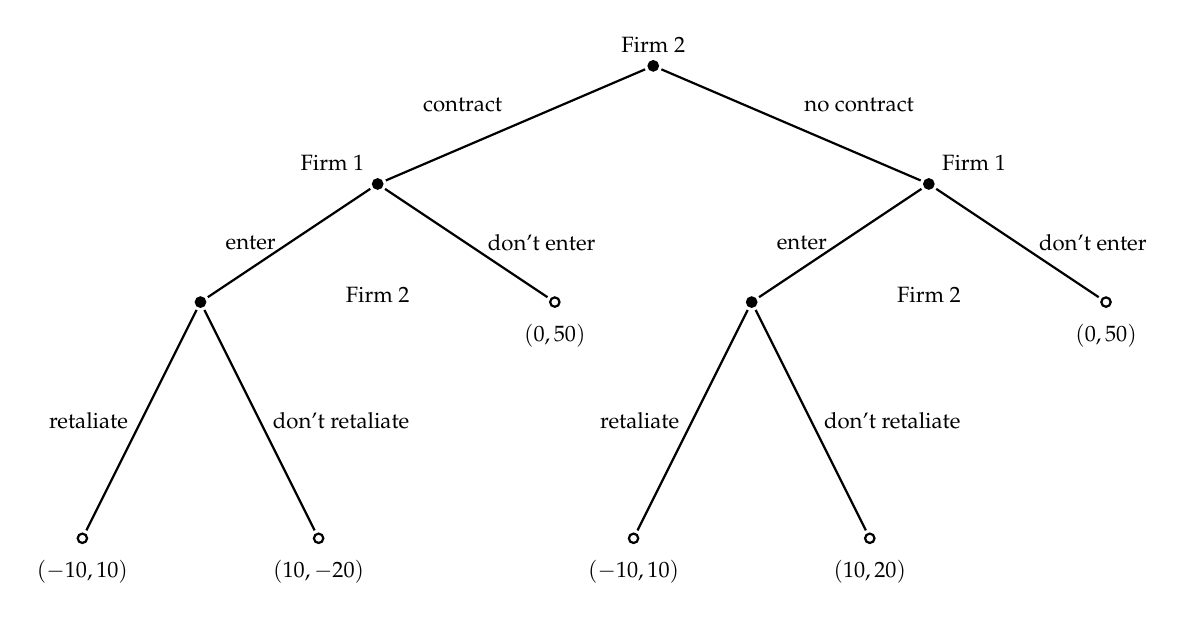
\begin{tikzpicture}[scale=1,font=\footnotesize]
	% Two node styles: solid and hollow
	\tikzstyle{solid node}=[circle,draw,inner sep=1.2,fill=black];
	\tikzstyle{hollow node}=[circle,draw,inner sep=1.2];
	% Specify spacing for each level of the tree
	\tikzstyle{level 1}=[level distance=15mm,sibling distance=70mm]
	\tikzstyle{level 2}=[level distance=15mm,sibling distance=45mm]
	\tikzstyle{level 3}=[level distance=30mm,sibling distance=30mm]
	% The Tree
	\node(0)[solid node]{}
	child{node(1)[solid node]{}
		child{node[solid node]{}
			child{node[hollow node,label=below:{$(-10,10)$}]{} edge from parent node[left]{retaliate}}
			child{node[hollow node,label=below:{$(10,-20)$}]{} edge from parent node[right]{don't retaliate}}
			edge from parent node[left]{enter}
		}
		child{node[hollow node,label=below:{$(0,50)$}]{}
			edge from parent node[right, xshift=3]{don't enter}
		}
		edge from parent node[above left]{contract}
	}
	child{node(2)[solid node]{}
	child{node[solid node]{}
		child{node[hollow node,label=below:{$(-10,10)$}]{} edge from parent node[left]{retaliate}}
		child{node[hollow node,label=below:{$(10,20)$}]{} edge from parent node[right]{don't retaliate}}
		edge from parent node[left]{enter}
	}
	child{node[hollow node,label=below:{$(0,50)$}]{}
		edge from parent node[right, xshift=3]{don't enter}
	}
	edge from parent node[above right]{no contract}
	}
	;
	% specify movers
	\node[above]at(0){Firm 2};
	\node at ($.5*(1-1)+.5*(1-2)$) {Firm 2};
	\node at ($.5*(2-1)+.5*(2-2)$) {Firm 2};
	\node[above left]at(1){Firm 1};
	\node[above right]at(2){Firm 1};
	%\node[above right]at(0-3){$P2$};
	% payoffs
\end{tikzpicture}
\end{frame}

\begin{frame}{Sequential games: the value of commitment}
	\begin{wideitemize}
		\item The subgame-perfect Nash equilibrium of the previous game is (don't enter, retaliate) and firm 2 now gets a payoff of 50.
		\item This relied on the (credible) commitment to play retaliate if firm 1 entered.
		\item This is an example of a broader category of firm strategies called \textbf{entry deterrence}
	\end{wideitemize}
\end{frame}

\begin{frame}{Sequential games: the value of commitment}
	\begin{wideitemize}
		\item Two points:
		\item 1. A \textbf{credible commitment} may have significant strategic value
		\item 2. If we believe that firm 2 is credibly committed to playing retaliate then we could equivalently reformulate the game \textit{with player 2 moving first} (see next slide...)
	\end{wideitemize}
\end{frame}

\begin{frame}{Sequential games: the value of commitment}
	% Node styles
	\tikzset{
		% Two node styles for game trees: solid and hollow
		solid node/.style={circle,draw,inner sep=1.5,fill=black},
		hollow node/.style={circle,draw,inner sep=1.5}
	}
	
	\begin{columns}[onlytextwidth, T] 
		\begin{column}{.55\textwidth}
			\begin{tikzpicture}[scale=1.5,font=\footnotesize]
				% Specify spacing for each level of the tree
				\tikzstyle{level 1}=[level distance=15mm,sibling distance=35mm]
				\tikzstyle{level 2}=[level distance=15mm,sibling distance=15mm]
				% The Tree
				\node(0)[solid node,label=above:{Firm 2}]{}
				child{node(1)[solid node]{}
					child{node[hollow node,label=below:{$(-10,10)$}]{} edge from parent node[left]{enter}}
					child{node[hollow node,label=below:{$(0,50)$}]{} edge from parent node[right]{don't enter}}
					edge from parent node[left,xshift=-3]{retaliate}
				}
				child{node(2)[solid node]{}
					child{node[hollow node,label=below:{$(10,20)$}]{} edge from parent node[left]{enter}}
					child{node[hollow node,label=below:{$(0,50)$}]{} edge from parent node[right]{don't enter}}
					edge from parent node[right,xshift=-3]{don't retaliate}
				};
				\node at ($(1)!.5!(2)$) {Firm 1};
			\end{tikzpicture}
		\end{column}
		\begin{column}{.4\textwidth}
			\begin{wideitemize}
				\item \textbf{Questions:}
				\item 1. Find the Nash equilibria
				\item 2. Find the subgame-perfect equilibria 
			\end{wideitemize}
		\end{column}
	\end{columns}
\end{frame}


\begin{frame}{Sequential games: the value of commitment}
	% Node styles
	\tikzset{
		% Two node styles for game trees: solid and hollow
		solid node/.style={circle,draw,inner sep=1.5,fill=black},
		hollow node/.style={circle,draw,inner sep=1.5}
	}
	
	\begin{columns}[onlytextwidth, T] 
		\begin{column}{.55\textwidth}
			\begin{tikzpicture}[scale=1.5,font=\footnotesize]
				% Specify spacing for each level of the tree
				\tikzstyle{level 1}=[level distance=15mm,sibling distance=35mm]
				\tikzstyle{level 2}=[level distance=15mm,sibling distance=15mm]
				% The Tree
				\node(0)[solid node,label=above:{Firm 2}]{}
				child{node(1)[solid node]{}
					child{node[hollow node,label=below:{$(-10,10)$}]{} edge from parent node[left]{enter}}
					child{node[hollow node,label=below:{$(0,50)$}]{} edge from parent node[right]{don't enter}}
					edge from parent node[left,xshift=-3]{retaliate}
				}
				child{node(2)[solid node]{}
					child{node[hollow node,label=below:{$(10,20)$}]{} edge from parent node[left]{enter}}
					child{node[hollow node,label=below:{$(0,50)$}]{} edge from parent node[right]{don't enter}}
					edge from parent node[right,xshift=-3]{don't retaliate}
				};
				\node at ($(1)!.5!(2)$) {Firm 1};
			\end{tikzpicture}
		\end{column}
		\begin{column}{.4\textwidth}
			\begin{wideitemize}
				\item \textbf{Questions:}
				\item 1. Find the Nash equilibria (enter, don't retaliate), (don't enter, retaliate)
				\item 2. Find the subgame-perfect equilibria (don't enter, retaliate)
			\end{wideitemize}
		\end{column}
	\end{columns}
\end{frame}

\begin{frame}{Sequential games: the value of commitment}
	\begin{wideitemize}
		\item We used \textbf{entry deterrence} as an example of the value of commitment. 
		\item Some other examples (beyond just economics)
		\item Dr Strangelove/Mutually Assured Destruction
		\item Rebel Without A Cause; how to win games of chicken
	\end{wideitemize}
		\begin{figure}
					\includegraphics[scale=1.0]{chicken.jpeg}
		\end{figure}
\end{frame}

\begin{frame}{Sequential games: long-run vs short-run}
	\begin{wideitemize}
		\item Sequential behavior arises naturally as well when thinking about short-run vs long-run decisions. We will see this later in the course.
		\item E.g. first choose (long-run) investment in capacity, second, choose (short-run) prices
	\end{wideitemize}
\end{frame}

\begin{frame}{Plan}
	\begin{wideenumerate}
		\item Sequential games: setup and equilibrium
		\item Sequential games: the value of commitment
		\item  \textbf{Sequential games: rationality assumption}
	\end{wideenumerate}
\end{frame}

\begin{frame}{Sequential games: rationality assumption}
	\begin{wideitemize}
		\item To what extent should we believe the predictions from sequential games?
		\item Similar to simultaneous games, we need to make predictions about what strategies other players will choose, and to do this we implicitly assume other players are \textit{rational} (they will correctly be able to solve the game etc..)
		\item When might we be worried about this assumption? 
	\end{wideitemize}
\end{frame}

\begin{frame}{Sequential games: rationality assumption - centipede game}
	\begin{figure}
	\centering
	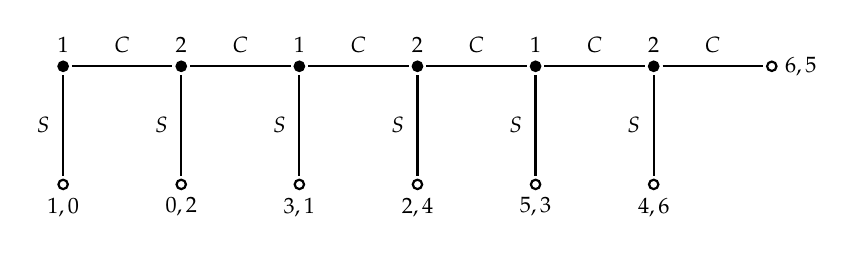
\begin{tikzpicture}[font=\footnotesize,scale=1]
		% Two node styles: solid and hollow
		\tikzstyle{solid node}=[circle,draw,inner sep=1.2,fill=black];
		\tikzstyle{hollow node}=[circle,draw,inner sep=1.2];
		% The Tree
		\node(0)[solid node]{}
		child[grow=down]{node[hollow node]{}edge from parent node[left]{$S$}}
		child[grow=right]{node(1)[solid node]{}
			child[grow=down]{node[hollow node]{}edge from parent node[left]{$S$}}
			child[grow=right]{node(2)[solid node]{}
				child[grow=down]{node[hollow node]{}edge from parent node[left]{$S$}}
				child[grow=right]{node(3)[solid node]{}
					child[grow=down]{node[hollow node]{}edge from parent node[left]{$S$}}
					child[grow=right]{node(4)[solid node]{}
						child[grow=down]{node[hollow node]{}edge from parent node[left]{$S$}}
						child[grow=right]{node(5)[solid node]{}
							child[grow=down]{node[hollow node]{}edge from parent node[left]{$S$}}
							child[grow=right]{node(6)[hollow node]{}
								edge from parent node[above]{$C$}
							}
							edge from parent node[above]{$C$}
						}
						edge from parent node[above]{$C$}
					}
					edge from parent node[above]{$C$}
				}
				edge from parent node[above]{$C$}
			}
			edge from parent node[above]{$C$}
		};
		% Movers
		Page 23 of 28
		\foreach \x in {0,2,4}
		\node[above]at(\x){1};
		\foreach \x in {1,3,5}
		\node[above]at(\x){2};
		% payoffs
		\node[below]at(0-1){$1,0$};
		\node[below]at(1-1){$0,2$};
		\node[below]at(2-1){$3,1$};
		\node[below]at(3-1){$2,4$};
		\node[below]at(4-1){$5,3$};
		\node[below]at(5-1){$4,6$};
		\node[right]at(6){$6,5$};
	\end{tikzpicture}
	\vspace{22pt}
	\end{figure}
	\begin{wideitemize}
		\item 1. Solve this game by backwards induction
		\item 2. Is this equilibrium reasonable?
		\item 3. What are the implicit rationality assumptions?
	\end{wideitemize}
\end{frame}

\begin{frame}{Sequential games: rationality assumption - centipede game}
	\begin{figure}
		\centering
		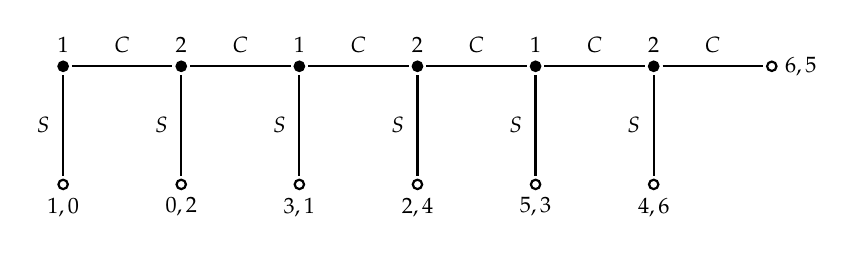
\begin{tikzpicture}[font=\footnotesize,scale=1]
			% Two node styles: solid and hollow
			\tikzstyle{solid node}=[circle,draw,inner sep=1.2,fill=black];
			\tikzstyle{hollow node}=[circle,draw,inner sep=1.2];
			% The Tree
			\node(0)[solid node]{}
			child[grow=down]{node[hollow node]{}edge from parent node[left]{$S$}}
			child[grow=right]{node(1)[solid node]{}
				child[grow=down]{node[hollow node]{}edge from parent node[left]{$S$}}
				child[grow=right]{node(2)[solid node]{}
					child[grow=down]{node[hollow node]{}edge from parent node[left]{$S$}}
					child[grow=right]{node(3)[solid node]{}
						child[grow=down]{node[hollow node]{}edge from parent node[left]{$S$}}
						child[grow=right]{node(4)[solid node]{}
							child[grow=down]{node[hollow node]{}edge from parent node[left]{$S$}}
							child[grow=right]{node(5)[solid node]{}
								child[grow=down]{node[hollow node]{}edge from parent node[left]{$S$}}
								child[grow=right]{node(6)[hollow node]{}
									edge from parent node[above]{$C$}
								}
								edge from parent node[above]{$C$}
							}
							edge from parent node[above]{$C$}
						}
						edge from parent node[above]{$C$}
					}
					edge from parent node[above]{$C$}
				}
				edge from parent node[above]{$C$}
			};
			% Movers
			Page 23 of 28
			\foreach \x in {0,2,4}
			\node[above]at(\x){1};
			\foreach \x in {1,3,5}
			\node[above]at(\x){2};
			% payoffs
			\node[below]at(0-1){$1,0$};
			\node[below]at(1-1){$0,2$};
			\node[below]at(2-1){$3,1$};
			\node[below]at(3-1){$2,4$};
			\node[below]at(4-1){$5,3$};
			\node[below]at(5-1){$4,6$};
			\node[right]at(6){$6,5$};
		\end{tikzpicture}
		\vspace{22pt}
	\end{figure}
	\begin{wideitemize}
		\item 1. Solve this game by backwards induction: Play S at each node
		\item 2. Is this equilibrium reasonable?: Maybe not... (in experiments, people tend to play C at each node)
		\item 3. What are the implicit rationality assumptions? That both players solve the game with backwards induction.
	\end{wideitemize}
\end{frame}

\begin{frame}{Summary of key points*}
	%\vspace{-20pt}
	\begin{wideitemize}
		\item Know how to identify the components of a sequential game
		\item Know how to compute the equilibrium of a sequential game via backwards induction
		\item Convert a sequential game to normal form and vice-versa
		\item Understand the pre-commitment may be valuable because it makes threats credible (e.g. in entry deterrence)
		\item Understand the implicit assumption of rationality that we make when solving sequential games
	\end{wideitemize}
	\vspace{20pt}
	*To clarify, all the material in the slides, problem sets, etc is assessable unless stated otherwise, but I hope this summary might be a useful place to start when studying the material.
\end{frame}

\begin{frame}{Ex. 7.7 HDTV Standards}
	\begin{wideitemize}
		\item \textbf{Question:} US and Japan simultaneously decide whether to invest a high or low value into HDTV research. If both countries choose `low' payoffs are (4,3) for the US and Japan respectively. If US chooses low level and Japan a high level, payoffs are (2,4). If US chooses high level and Japan low, payoffs are (3,2). If both countries chooses a high level, payoffs are (1,1). 
		\item 1. Are there any dominant strategies in this game? What is the Nash equilibrium? What are the implicit rationality assumptions?
		\item 2. Suppose the US now has the option of committing to a strategy ahead of Japan. How would you model this situation? What are the subgame-perfect Nash equilbria of this game?
		\item 3. Comparing your answers to 1. and 2., what can you say about the value of commitment for the US?
	\end{wideitemize}
\end{frame}

\begin{frame}{Price match guarantee in the market for luxury cars}
	\begin{wideitemize}
		\item Two firms are competing on prices. Each firm can choose to set a high price $p_H$ or a low price $p_L$, where $p_H > p_L$. Profits are given by:
		\begin{figure}
			\centering
		 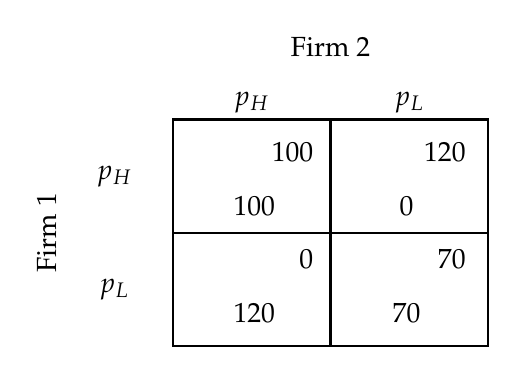
\begin{tikzpicture}
			\matrix[matrix of math nodes,every odd row/.style={align=right},every evenrow/.style={align=left},every node/.style={text width=1.5cm},row sep=0.2cm,column sep=0.2cm,ampersand replacement=\&] (m) {
				100 \& 120 \\
				100 \& 0 \\
				0 \& 70 \\
				120 \& 70 \\
			};
			\draw (m.north east) rectangle (m.south west); 
			\draw (m.north) -- (m.south);
			\draw (m.east) -- (m.west);
			
			% Player 1
			\coordinate (c) at ($(m.north west)!0.25!(m.south west)$);
			\coordinate (d) at ($(m.north west)!0.75!(m.south west)$);
			\node[left=2pt of c,text width=1cm]  {$p_H$};
			\node[left=2pt of d,text width=1cm]  {$p_L$};
			
			% Player 2
			\coordinate (a) at ($(m.north west)!0.25!(m.north east)$);
			\coordinate (b) at ($(m.north west)!0.75!(m.north east)$);
			\node[above=5pt of a,anchor=base] {$p_H$};
			\node[above=5pt of b,anchor=base] {$p_L$};
			
			\node[above=18pt of m.north] (firm b) {Firm 2};
			\node[left=1.6cm of m.west,rotate=90,align=center,anchor=center] {Firm 1};
			
			%\node[above=5pt of firm b]  {Payoff Matrix};
		\end{tikzpicture}
		\end{figure}
		\begin{wideitemize}
		\item 1. Draw the extensive form if firm 1 moves first. Solve for the subgame perfect equilibrium.
		\item 2. Suppose firm 1 offers consumers to match its price with the lowest price in the market. Solve for the SPE of the modified game (Hint: modify the game to three stages, allowing firm 1 to make a move in the third stage only in the case where it chose $p_H$ in the firms stage and firm 2 chose $p_L$ in the second stage.)
		\end{wideitemize}
	\end{wideitemize}
\end{frame}

\end{document}
